\chapter{Background}
\label{ch:background}

\section{Artificial Neural  Networks}
\label{sec:ann}
An artificial neural network (ANN)  \cite{rashid2016make} \cite{youtube3blue1brown}  \cite{zhang2023dive} describes the architecture of neurons and their connection,  which is orientated towards biological neurons to simulate a learning process. 

ANNs consist of multiple layers, each of them containing a large number of neurons. The input layer consists of a node for each part of its input (e.g., a greyscale picture with the size of 400 x 400 pixels could contain 160,000 input nodes, one node for each pixel with an input between 0 and 255). The output layer is the last layer where the number of neurons maps directly to the desired output (e.g., if you want to decide if the animal in the picture is a dog or a cat, you could use one final neuron - if it activated, the ANN detected a cat, otherwise a dog). All layers in between are called hidden layers because they are not influenced by the outside. Each neuron has an activation function, determining if a neuron is activated by its input. Every neuron in layer $k$ can get its input from other neurons' output from the layer $k-1 = j$. An edge between two neurons has a weight $w^{jk}$ assigned, influencing the sum of all the inputs from this edge. In mathematical terms, an artificial neuron is described by a function, also called an activation function. Over a layer's potentials and weights of the edges, a weighted sum is formed and projected via the activation function into a smaller space. Two often used functions are the Sigmoid function which projects all values into the interval $(0, 1)$
\begin{equation}
{\phi (\mathbf{v} )=(1+\exp(- \mathbf {v}))^{-1}}
\end{equation}  
and the ReLU function, projecting to $[0, \infty)$:
\begin{equation}
\phi (\mathbf{v}) = \max(0, \mathbf{v})
\end{equation}.
Also, a bias ($\beta$) could be added to shift neurons activation potential. 

To calculate the output of a neural network, a neuron's activation potential could be written down as a vector, multiplied by a matrix containing every edge that leads to the nodes in layer $k$. One row in the matrix corresponds to the edges between a neuron in layer $j$ and a particular neuron in layer $k$. After that, a bias is added, and everything is wrapped into an activation function again, leading to the next node's potential \cite{youtube3blue1brown} \cite{zhang2023dive}:
\begin{equation}
\label{eq:ann_forward_propergation}
\boldsymbol{H}^{k} = \phi \left(
\begin{bmatrix}
w^{jk}_{0,0} & w^{jk}_{0,1} & \cdots & w^{jk}_{0,m}\\
w^{jk}_{1,0} & w^{jk}_{1,1} & \cdots & w^{jk}_{1,m}\\
\vdots  & \vdots  & \ddots & \vdots \\
w^{jk}_{n,0} & w^{jk}_{n,1} & \cdots & w^{jk}_{n,m} \\
\end{bmatrix}
\cdot
\begin{bmatrix}
a_{0}^{j}\\
a_{1}^{j}\\
\vdots \\
a_{2}^{j}\\
\end{bmatrix}
+
\begin{bmatrix}
\beta_{0}^{j}\\
\beta_{1}^{j}\\
\vdots \\
\beta_{2}^{j}\\
\end{bmatrix}
\right) 
\xrightarrow{\text{}}
\boldsymbol{H}^{k} = \phi{(\boldsymbol{W}^{jk}\boldsymbol{A}^j + \boldsymbol{\beta}^j)}
\end{equation}
To make ANNs effective in predicting outputs, they have to be trained. "Backpropagation" describes the process of training the model to minimize the total cost by each output (or batch). For every result, the cost (also called "loss" or "error") in the output layer $c_n$ is calculated by subtracting the actual output $a_n$ from node $n$ by the expected output $e_n$. Squaring the result for an individual node and taking the sum over all nodes results in the cost of one run. For all nodes, the cost is:
\begin{equation}
\vect{c} = 
\begin{bmatrix}
(e_{1} - a_{1})^{2}\\
(e_{2} - a_{2})^{2}\\
\vdots \\
(e_{n} - a_{n})^{2}\\
\end{bmatrix}
\end{equation}
The average cost of multiple runs describes the performance of a neural network. 
Finding the global minimum of the cost function could be an option to minimize the cost. The problem with this approach is that the calculation cost is too high, making even calculations for small networks inefficient. Therefore, "gradient descent" is used, which approaches a local minimum iteratively. For backpropagation, the sensitivity of the cost function for a neuron with respect to every connected weight (and biases) is interesting because it represents the slope of the error function. The question is, how much do the weights of the edges have to be changed to correct the output. Mathematically speaking \cite{zhang2023dive}, this is denoted by:

\begin{equation}
\frac{\partial{\vect{c}}}{\partial{\boldsymbol{W}^{jk}}}
\end{equation}
Looking at the network error function with the idea in mind that only the errors from the nodes that the neuron is connected to is interesting, the formula can be reformulated to: 

\begin{equation}
\frac{\partial{\vect{c}}}{\partial{\boldsymbol{W}^{jk}}} = \frac{\partial}{\partial{\boldsymbol{W}^{jk}}} +  \vect{c}^k
\end{equation}
As mentioned above the indices $j$ and $k$ reference the different layers, where $\boldsymbol{W}^{jk}$ is a matrix containing the weights connecting layer $j$ and $k$. In the calculation, it is also assumed that $k$ represents the final layer. Looking at $\vect{c}^k$, it is known that $\vect{e}^k$, the expected output, is not dependent on the function. With the chain rule and building the resulting derivatives, the following term emerges:

\begin{equation}
\frac{\partial{\vect{c}}}{\partial{\boldsymbol{W}^{jk}}} = \frac{\partial{\vect{c}}}{\partial{\vect{a}^k}}
\cdot \frac{\partial{\vect{a}^k}}{\partial{\boldsymbol{W}^{jk}}} = -2\vect{c}^k \cdot \frac{\partial{\vect{a}^k}}{\partial{\boldsymbol{W}^{jk}}}
\end{equation}

The second part of the equation heavily depends on the activation function because $a^k$ is the activation of the node in layer $k$, in this case, in the final layer, and is calculated by $\phi(\sum_j \boldsymbol{W}^{jk} \cdot \vect{a}^j)$. Calculating the derivative of the last term with the chain rule results in:

\begin{equation}
\frac{\partial{\vect{c}}}{\partial{\boldsymbol{W}^{jk}}}
= -2\vect{c}^{k} \cdot \phi'\left(\sum_j \boldsymbol{W}^{jk} \cdot \vect{a}^j\right) \cdot \frac{\partial}{\partial{\boldsymbol{W}^{jk}}} \vect{a}^k 
= -2\vect{c}^{k} \cdot \phi'\left(\sum_j \boldsymbol{W}^{jk} \cdot \vect{a}^j\right) \cdot \vect{a}^j
\end{equation}
This is the formula to calculate the change for the weights connecting the output. With the small modification of removing the factor $2$ (when adding the direction to the weight later, it is scaled via a new factor also called "learning rate") and looking at $\vect{c}^k$ as the error of layer $k$ (which is calculated by taking multiplying the transformed nodes from any layer $k$ with the weights from $jk$), with $j$ and $k$ being an arbitrary layer, this results in the final function for updating the weights:
\begin{equation}
\frac{\partial{\vect{c}}}{\partial{\boldsymbol{W}^{jk}}}
= -\vect{c}^{k} \cdot \phi'\left(\sum_j \boldsymbol{W}^{jk} \cdot \vect{a}^j\right) \cdot \vect{a}^{j}
\end{equation}
For updating weights, the calculation is
\begin{equation}
\boldsymbol{W}^{jk} = \boldsymbol{W}^{jk} - \alpha \cdot \frac{\partial{\vect{c}}}{\partial{\boldsymbol{W}^{jk}}} 
\end{equation}
with $\alpha$ being the above-mentioned learning rate. Implementing such a neural network heavily relies on matrix multiplications which can be calculated very efficiently, especially with the help of modern graphic cards. Because of this, ANNs are in use to this day, often in combination with other network types that are presented below \cite{yolox2021} \cite{vaswani2023attentionneed}.

\section{Convolutional Neural Networks}
Conventional Neural networks (CNNs) \cite{oshea2015introductionconvolutionalneuralnetworks} are another type of network and are often combined with ANNs. They are used to extract features from an image by applying different "filters" to it. 

A CNN consists of multiple layers as well. Like an ANN, a CNN typically includes an input layer with a size corresponding to the number of pixels in the input image and maps to a much smaller number of nodes. In a CNN, the activation of a neuron depends on a learnable kernel. A kernel is a matrix that convolves over the input vector, aiming to extract important features while diminishing unimportant ones. Convolution involves selecting a pooled vector $\boldsymbol{p}$, usually represented as a quadratic matrix $\boldsymbol{P}$ with a center value $c$, and a quadratic kernel $\boldsymbol{K}$. The pooled vector and kernel are multiplied together via the dot product, with the resulting value replacing $c$ in the input vector. Through backpropagation, the kernel is trained to improve performance. \cite{oshea2015introductionconvolutionalneuralnetworks}

Due to performance reasons, a CNN is often used to map a large input to a smaller dimension by adjusting the depth, the stride, and zero padding. Depth describes the number of convolution layers (a reduction leads to fewer neurons for the cost of recognition performance), the stride is the distance around different center points, and zero-padding is the \textit{"simple process of padding the border of the input"} \cite{oshea2015introductionconvolutionalneuralnetworks}.

Another way to reduce the output size is by using a pooling layer. In pooling layers, a kernel (typically 2 x 2) is used with a larger stride than $\frac{width_{\text{kernel}}}{2}$ to further minimize the output array. Only the largest number within the pooled vector is carried to the next layer for max pooling. Pooling layers can also be used for other optimizations, such as L1/L2 normalization \cite{Wu_2019} \cite{gholamalinezhad2020poolingmethodsdeepneural} and average pooling \cite{gholamalinezhad2020poolingmethodsdeepneural} \cite{oshea2015introductionconvolutionalneuralnetworks}.

\section{Autoencoder}
\label{sec:autoencoder}
The Autoencoder architecture describes a possible solution for compressing high dimensional data to lower dimensions (encoder) and rebuilding it with information, the encoder removed (decoder). The idea was first proposed in the paper "Fully Convolutional Networks for Semantic Segmentation" \cite{long2015fullyconvolutionalnetworkssemantic} as an efficient upsampling method after downsizing an image by a CNN.

As mentioned above, autoencoders reduce their input to a much smaller space, known as the "latent space". It later upscales the vector in the smaller space again to a possible new domain, such as segmentation maps for image classification. The downscaling/encoding is performed by a CNN, consisting of multiple kernel and pooling layers. In modern autoencoders, these memorized pooled indices are filtered by a \textit{"trainable filter bank"}\cite{badrinarayanan2015segnetdeepconvolutionalencoderdecoder} and later injected into the decoding process to get lost information by the encoding process back into the image. The decoder is also a CNN with small modifications, often called a "deconvolution network". Instead of convolution, deconvolution takes a smaller input and expands it into a larger output with the help of a trainable kernel. The pooling layers are reversed with the help of the filter bank.

An implementation of this approach, which is used to this day is the "UNET" \cite{ronneberger2015unetconvolutionalnetworksbiomedical}. For the encoder part the network uses \textit{"two 3x3 convolutions (unpadded convolutions), each followed by
a rectified linear unit (ReLU) and a 2x2 max pooling operation with stride 2"} \cite{ronneberger2015unetconvolutionalnetworksbiomedical} doubling the number of feature channels (each kernel produces an output for each input, which results in $\text{fchannels}_{\text{output}} = 2 \cdot \text{fchannels}_{\text{input}}$). The decoder part reverses this process, but instead of injecting the data via a "filter bank", it concatenates the corresponding feature map to each layer. It bisects it afterward via deconvolution. That results in the decoder side having one additional convolution, reducing the "feature channels" without any concatenation to its final result.

\begin{figure}[H]
  \centering
  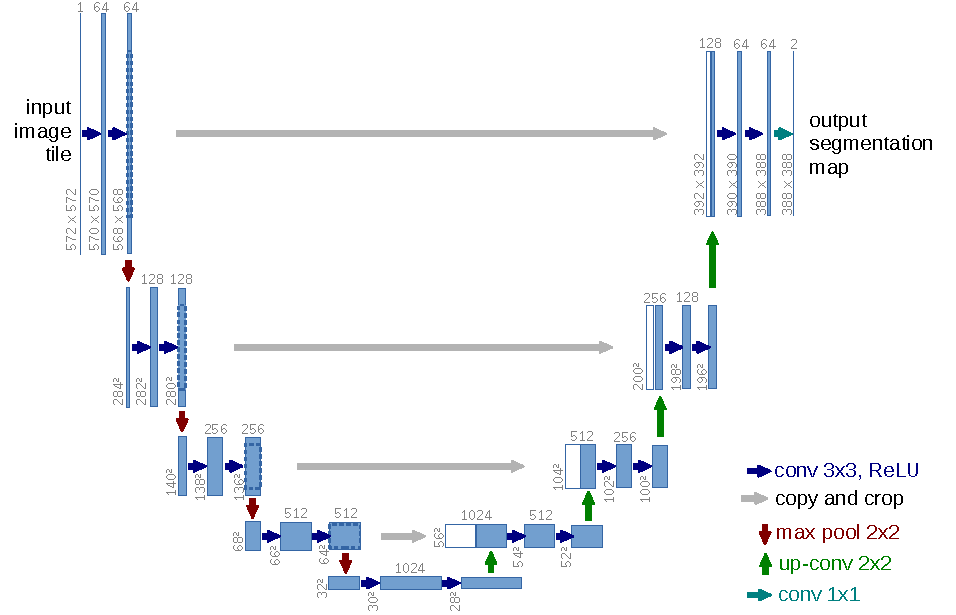
\includegraphics[width=\textwidth]{figures/background/u-net-illustration-correct-scale2.pdf}
  \caption{Structure of the UNET architecture. \cite{ronneberger2015unetconvolutionalnetworksbiomedical}}
  \label{fig:unet}
  \clearpage
\end{figure}

\section{GAN}
\label{sec:gan}
Generative Adversarial Net (GAN) \cite{goodfellow2014generativeadversarialnetworks} is an architecture for generating and validating images through a second instance. A generative model, $G$, and a discriminative model, $D$ are trained together with $G$ generating data to fool $D$. $D$ distinguishes between "real" (Data from the training set) and generated, often called "fake" data. Both models are trained using backpropagation, avoiding complex inference methods. Various experiments demonstrate \cite{zhao2024exploring} \cite{karras2018progressivegrowinggansimproved} that this adversarial process drives $G$ to produce realistic data. 

This raises the question: what are the advantages of playing such a game, and why not simply predict every pixel individually to produce a completed picture? This approach also exists, and these frameworks are called "Autoregressors" \cite{oord2016pixelrecurrentneuralnetworks}. They can be trained by removing information from an image and letting the model predict the missing information. The problem with this approach lies in the complexity of image generation. While generating embedding after embedding up to a few hundred is fine, generating a few million pixels is slow. The problem with developing a more significant number of pixels simultaneously is that Neuronal networks average their output, resulting in a blurry result. 

GANs, therefore, play their adversarial game with the discriminator, allowing generation in one passthrough starting with a random vector.

Looking at the adverse game inside a GAN from a mathematical perspective, to calculate the loss for such a framework, the following value function is important: \cite{goodfellow2014generativeadversarialnetworks}:

\begin{equation}
\label{eq:minimaxgame-definition}
\mathcal{L} = \min_G \max_D V(D, G) = \mathbb{E}_{x \sim p_{\text{data}}(x)}[\log D(x)] + \mathbb{E}_{z \sim p_{z}(z)}[\log (1 - D(G(z)))]
\end{equation}

where $G$ marks a parameterized function and $D$ the discriminator, a function returning a scalar. The first part of the equation

\begin{equation}
\min_G \max_D V_I(D, G) = \mathbb{E}_{x \sim p_{\text{data}}(x)}[\log D(x)]
\end{equation}

maximizes $D$ for a given element from the data, and the second part

\begin{equation}
\min_G \max_D V_{II}(D, G) = \mathbb{E}_{z \sim p_{z}(z)}[\log (1 - D(G(z)))]
\end{equation}

minimizes $D$ for $G$ from $D$'s perspective and maximizes $D$ from $G$'s perspective if the image is a "fake". 


\section{Recurrent Neural Networks}

Recurrent Neural Networks (RNN) \cite{zhang2023dive} enlarge ANNs by allowing each neuron to input its previous output again and thus maintain its state. Therefore, RNNs are well-suited for tasks like natural language processing, time series prediction, and speech recognition.

Looking into this from a mathematical point of view, the goal is to predict a token $x$ at time $t$ with a set of tokens that were injected into the model before $t$. They are denoted as $x_{t - n}$ with $n \in \mathbb{N} \land t - n > 0$. Because it would be computationally too expensive to store a state of the network for each token, all of them are combined into a hidden state $h$. A hidden state is defined as a state inside a neuronal network that can only be calculated recursively on top of the previous result:

\begin{equation}
\mathbb{P}(x_t | x_{t - 1}, ..., x_0) \approx \mathbb{P}(x_t | h_{t-1})
\end{equation}
Extending \autoref{eq:ann_forward_propergation} by the inner state with extra weights for control leads to: 

\begin{equation}
    \boldsymbol{H}_t = \phi{(\boldsymbol{W}_{l}^{j-1}\boldsymbol{A} + \boldsymbol{W}_{s}^{j}\boldsymbol{H}_{t-1} + \boldsymbol{\beta}^{j-1})}
\end{equation}
One of the problems of this approach is that for each iteration the weight $\boldsymbol{W}_{s}^{j}$ is multiplied again to $\boldsymbol{H}$. If this weight is larger than $1$, over time, it leads to large gradients, also called gradient explosion. On the other hand, if it is smaller than $1$, it leads to gradient vanishing \cite{zhang2023dive}. For that reason, RNNs were modified to different forms like long short-term memory \cite{zhang2023dive} \cite{hochreiter1997lstm} and gated recurrent networks \cite{chung2014empirical}, which use memory cells and gates to maintain and regulate information across long sequences.

\section{Transformer Models \& Self Attention}
\label{sec:transformer_models_and_self_attention}
As mentioned above, the biggest problems regarding recurrent neural networks are gradient vanishing and explosion and not memorizing features over a large context size \cite{zhang2023dive}. 
To counter this, attention was created, an approach that allows finding features in early tokens and memorizing them over a long time. It was combined into a transformer, a deep-learning architecture proposed by researchers at Google. This architecture, unlike its predecessors, only uses attention to maintain its state, which increases performance regarding translation tasks and later led to the creation of Large Language Models \cite{brown2020language}, as well as cross-attention and backbone architectures for latent diffusion algorithms
\cite{rombach2022highresolution} \cite{peebles2023scalablediffusionmodelstransformers}. 

A transformer has two different parts: an encoder and a decoder \autoref{sec:autoencoder}. In this architecture, the encoder and decoder have a defined size of stacks, where each stack is again divided into two sub-layers, with the first being a multi-head self-attention mechanism and the second being a simple, position-wise, fully connected feed-forward network \autoref{sec:ann}. The decoder adds a third sub-layer to each stack, which performs multi-head attention over the output of the encoder stack and also masks the output tokens to not influence previous ones.\cite{vaswani2023attentionneed}  

The core of the transformer model is the attention mechanism, which aims to enhance a token with the meanings of the other tokens around it. The idea is to map the tokens from the high dimensional embedding space to a smaller Query/Keyspace and multiply the attention pattern to the embedding. A query $\vect{q}_1$ is calculated by multiplying a matrix $\boldsymbol{W}_Q$, consisting of tunable parameters, with the token vector of an embedding $\boldsymbol{e_i}$. A key is calculated the same way, but instead of multiplying $\boldsymbol{W}_Q$ with the embedding, the key matrix $\boldsymbol{W}_K$, another matrix consisting of tunable parameters is used. After that, a new matrix is calculated by multiplying the dot product of each resulting key-value pair and multiplying it with the corresponding $\vect{v}_k$, resulting from multiplying another tunable matrix $\boldsymbol{W}_V$ by each embedding vector. $\boldsymbol{W}_V$ is normally split into two smaller matrices, as you can see later. \cite{vaswani2023attentionneed} \cite{youtube3blue1brown}

\begin{equation}
    \text{Attention}(\boldsymbol{Q}, \boldsymbol{K}, \boldsymbol{V}) = \text{softmax}\left(\frac{\boldsymbol{Q}\boldsymbol{K}^T}{\sqrt{d^k}}\right)\boldsymbol{V}
\end{equation}

$\boldsymbol{Q}$, $\boldsymbol{K}$ and $\boldsymbol{V}$ are vectors containing $[\boldsymbol{q}_1, \boldsymbol{q}_n]$, $[\boldsymbol{k}_1, \boldsymbol{k}_n]$ and $[\boldsymbol{v}_1, \boldsymbol{v}_n]$, while $\frac{1}{\sqrt{d^k}}$ counters the effect of the dot products growing large in magnitude and therefore \textit{"pushing the softmax function into regions where it has extremely small gradients"}. \cite{vaswani2023attentionneed}. As mentioned above, masking is also applied so that succeeding tokens do not influence previous tokens, as the goal of a transformer is to predict these. To preserve the normalized columns calculated by the softmax function, all entries in $\boldsymbol{Q}\boldsymbol{K}^T$ representing the influence of a succeeding token are set to infinity. \cite{vaswani2023attentionneed}

For each token, the influences resulting from $\text{Attention}(\boldsymbol{Q}, \boldsymbol{K}, \boldsymbol{V})$ are added up, resulting in $\Delta e_i$. This marks the change, which is added to $e_i$.

To make this idea computationally more efficient, these attention heads and their corresponding changes are calculated multiple times in parallel, each attention head with its own $\boldsymbol{Q}, \boldsymbol{K}, \boldsymbol{V}$:

\begin{multline}
    \text{MultiHead}(\boldsymbol{Q}, \boldsymbol{K}, \boldsymbol{V}) = \text{Concat}(head_1, ..., head_h)\boldsymbol{W}^{O}  \\ 
    \text{where } head_i = \text{Attention}(\boldsymbol{QW}^{Q}_{i} , \boldsymbol{KW}^{K}_{i}, \boldsymbol{VW}^{V}_{i} )
\end{multline}

where $\boldsymbol{W}^{O} \in \mathbb{R}^{hd_v \times d_\text{model}}$, $\boldsymbol{W}^{V} \in \mathbb{R}^{d_\text{model} \times d_v}$ and $h$ the number of attention layers. The previous matrix $\boldsymbol{W}^K$, which also exists $h$ times, is split up into $\boldsymbol{W}^{O}$ (also called Output Matrix) and $\boldsymbol{W}^{V}$, where only $\boldsymbol{W}^{V}$ is part of the attention mechanism. With this mechanism, calculating the weighted sums on the smaller matrices from $W^{O}$ and multiplying $W^{V}$ is much less computationally difficult.\cite{vaswani2023attentionneed} \cite{youtube3blue1brown} \cite{elhage2021mathematical}.

Every layer also consists of a Fast Forward Neuronal Network (FNN, a term equivalent to ANN \autoref{sec:ann}). The dimensions of this network's input and output layer are $d_\text{model}$. It also has a larger hidden layer, which in the implementation of this paper \cite{vaswani2023attentionneed} is scaled by factor $4$.

While transformer models' most famous usage today is in "Generative Pretrained Transformers" like GPT-3 \cite{brown2020language}, most diffusion algorithms, see \autoref{sec:latent_diffusion_models} use attention mechanisms to extract meaning out of text embeddings for image generations.

Also, despite one of the biggest problems Transformers have, being their context size growing by the factor ${\text{input}^2}$ ($\text{embeddings} \cdot \text{query}, \text{embeddings} \cdot \text{key}, \text{embeddings} \cdot \text{output-matrix}$), there are implementations of modern diffusion models using transformers to replace the UNET \cite{ronneberger2015unetconvolutionalnetworksbiomedical} \cite{peebles2023scalablediffusionmodelstransformers}.

\section{Latent Diffusion Models \& Text to Image}
\label{sec:latent_diffusion_models}

Instead of using GANs to generate high-quality images, (latent) diffusion models could also be used. The idea of diffusion models is to counter the blurring when generating too many images simultaneously by decoupling pixels so that they are independent of each other. This is done by adding random noise. Mathematically speaking, having an image $x_0$, in the encoding process, noise $\epsilon \sim  \mathcal{N}(0, 1)$ is applied $T$ times onto the image resulting in $x_T$. In every iteration, more noise gets added. The following interpolation can calculate each intermediate step $x_t$:

\begin{equation}
x_t = \left(\frac{T - t}{T}\right) \cdot \epsilon  + \left(1 - \frac{T - t}{T}\right) x_0
\end{equation}

The decoder is a function $\mathcal{E}_\theta$ with trained parameters to revert the noise added by the encoder step by step. This is done via the UNET \cite{peebles2023scalablediffusionmodelstransformers}, which is described above. To speed up this process during the training phase, evaluation of the result from denoising $x_t$ is not done against $x_t - 1$ but against $x_0$, or to be more exact, it predicts the noise $\epsilon_t$ until $\epsilon_0$. This is really efficient because that way, the model only learns how to denoise to a clean image and not all steps in between (this does not mean that denoising is done in one step later - it is only trained to do it in one step). Looking at the loss function, it is calculated as the "Mean Squared Error" between the actual noise applied and the current image $x_t$, which is, as mentioned above, put together out of noise $\epsilon_t$ and $x_0$.

The problems resulting from this approach are the long generation time (one denoising step equals one iteration through the network) and the large amount of training data needed to make the algorithm learn efficiently. To counter both of these problems, Robin Rombach proposed in his infamous paper "High-Resolution Image Synthesis with Latent Diffusion Models" \cite{rombach2022highresolution} to shift calculation from the pixel space to the latent space of the UNET, which is looking back at \autoref{fig:unet} at the bottom of the U-Shape.

To train the autoencoder, equivalent to the GAN approach (see \autoref{sec:gan}), a discriminator is used to distinguish between "fake" images produced by the autoencoder and the real images from the dataset - the resulting loss function from this approach now combines the diffusion loss function, the discriminator loss function and a third loss function, similar to the loss calculation of variational autoencoder (VAE) \cite{kingma2022autoencodingvariationalbayes}:

\begin{equation}
\mathcal{L}_{\text{Autoencoder}} =  \min_{\mathcal{E}, \mathcal{D}} \max_\psi \left( \mathcal{L}_{\text{rec}}(x, \mathcal{D}(\mathcal{E}(x))) - \mathcal{L}_{\text{adv}}(\mathcal{D}(\mathcal{E}(x))) + \log \mathcal{D}_\psi(x) + \mathcal{L}_{\text{reg}}(x; \mathcal{E}, \mathcal{D}) \right)
\label{eq:firststageloss}
\end{equation}

The diffusion loss is calculated in $\mathcal{L}_{\text{rec}}(x, \mathcal{D}(\mathcal{E}(x)))$, while $\mathcal{L}_{\text{reg}}(x; \mathcal{E}, \mathcal{D})$ is the regularisation of the latent image by taking the encoder output $\mathcal{E}(x) = L$, with $L$ being the image in the latent space and calculate the loss with respect to $\mathcal{N}(0, 1)$. The last two parts of this loss function 

\begin{equation}
\min_{\mathcal{E}, \mathcal{D}} \max_\psi \left(- \mathcal{L}_{\text{adv}}(\mathcal{D}(\mathcal{E}(x))) + \log \mathcal{D}_\psi(x)\right) 
\approx 
\min_{\mathcal{E}, \mathcal{D}} \max_\psi \left(\left[(\mathcal{D}_\psi(\mathcal{D}(\mathcal{E}(x)))) \right] + \log \mathcal{D}_\psi(x)\right)
\end{equation}
are part of the adverse game \autoref{sec:gan} and calculate the loss for minimizing the discriminator's output by adjusting the $\mathcal{D}_\psi$ (detecting that $(\mathcal{D}(\mathcal{E}(x)))$ is a "fake" image) while trying to maximize the discriminator's output by adjusting $(\mathcal{D}(\mathcal{E}(x)))$ (making $(\mathcal{D}(\mathcal{E}(x)))$ looks real). The last part, $\log \mathcal{D}_\psi(x)$, aims to maximize the discriminator's output for real images. Therefore, it is identical to the above described GAN loss function \autoref{eq:minimaxgame-definition}

Combining these two goals of the Latent Diffusion Model denoises the image to its state before and also prevents it from being detected by the discriminator, creating a well-defined latent space and allowing consistent image generation. Instead of running the denoising function $\mathcal{E}_\theta$ on the pixel-space representation $x_T$, it is more feasible to train and run it on the latent-space representation $z_T$ until $z_0$. The loss function is equivalent to the one on the pixel space. The resulting latent representation $z_0$ is afterward put into the decoder to obtain the final image.

The last important part of most of these models is the conditioning. Conditioning is done by concatenating the tokens with the images or by cross-attention. For cross-attention, the input is tokenized/split up (here defined as $\mathcal{T}_\theta$) equivalent to self-attention described in \autoref{sec:transformer_models_and_self_attention}. But instead of mapping tokens to itself, the latent image $z$ is mapped via the Query ${\boldsymbol{W}^{Q_z}}$ to the Keys $\boldsymbol{W}^{K_{\mathcal{T}_\theta}}$ and the Output $\boldsymbol{W}^{V_{\mathcal{T}_\theta}}$. To enhance the influence, classifier-free guidance \cite{ho2022classifierfreediffusionguidance}\cite{dieleman2022guidance} was introduced, where the image is generated two times, one time with and once without the condition, and only the difference is added:
\begin{equation}
z_i = z_{i + 1} + (\mathcal{E}_\theta(z_{i + 1} \oplus \mathcal{T}_\theta) - \mathcal{E}_\theta({z_{i + 1}}))
\end{equation}

Ultimately, the images can upscaled by latent diffusion models via conditioning \cite{rombach2022highresolution}. That allows the diffusion algorithm to generate the image on smaller inputs, resulting in higher calculation speed.

\section{ControlNet}
\label{ch:controlnet}

The ControlNet architecture \cite{zhang2023addingconditionalcontroltexttoimage} aims to enable latent diffusion models with additional conditioning inputs, avoiding the need to retrain parts of the original model, which would add significant computational costs. To achieve this, ControlNet duplicates the encoding layers of the diffusion network, treating each of them as a "trainable copy". The parameters of the original diffusion network are fixed, preventing any modifications, as symbolized by the lock in \autoref{fig:controlnet}.

\begin{figure}[H]
  \centering
  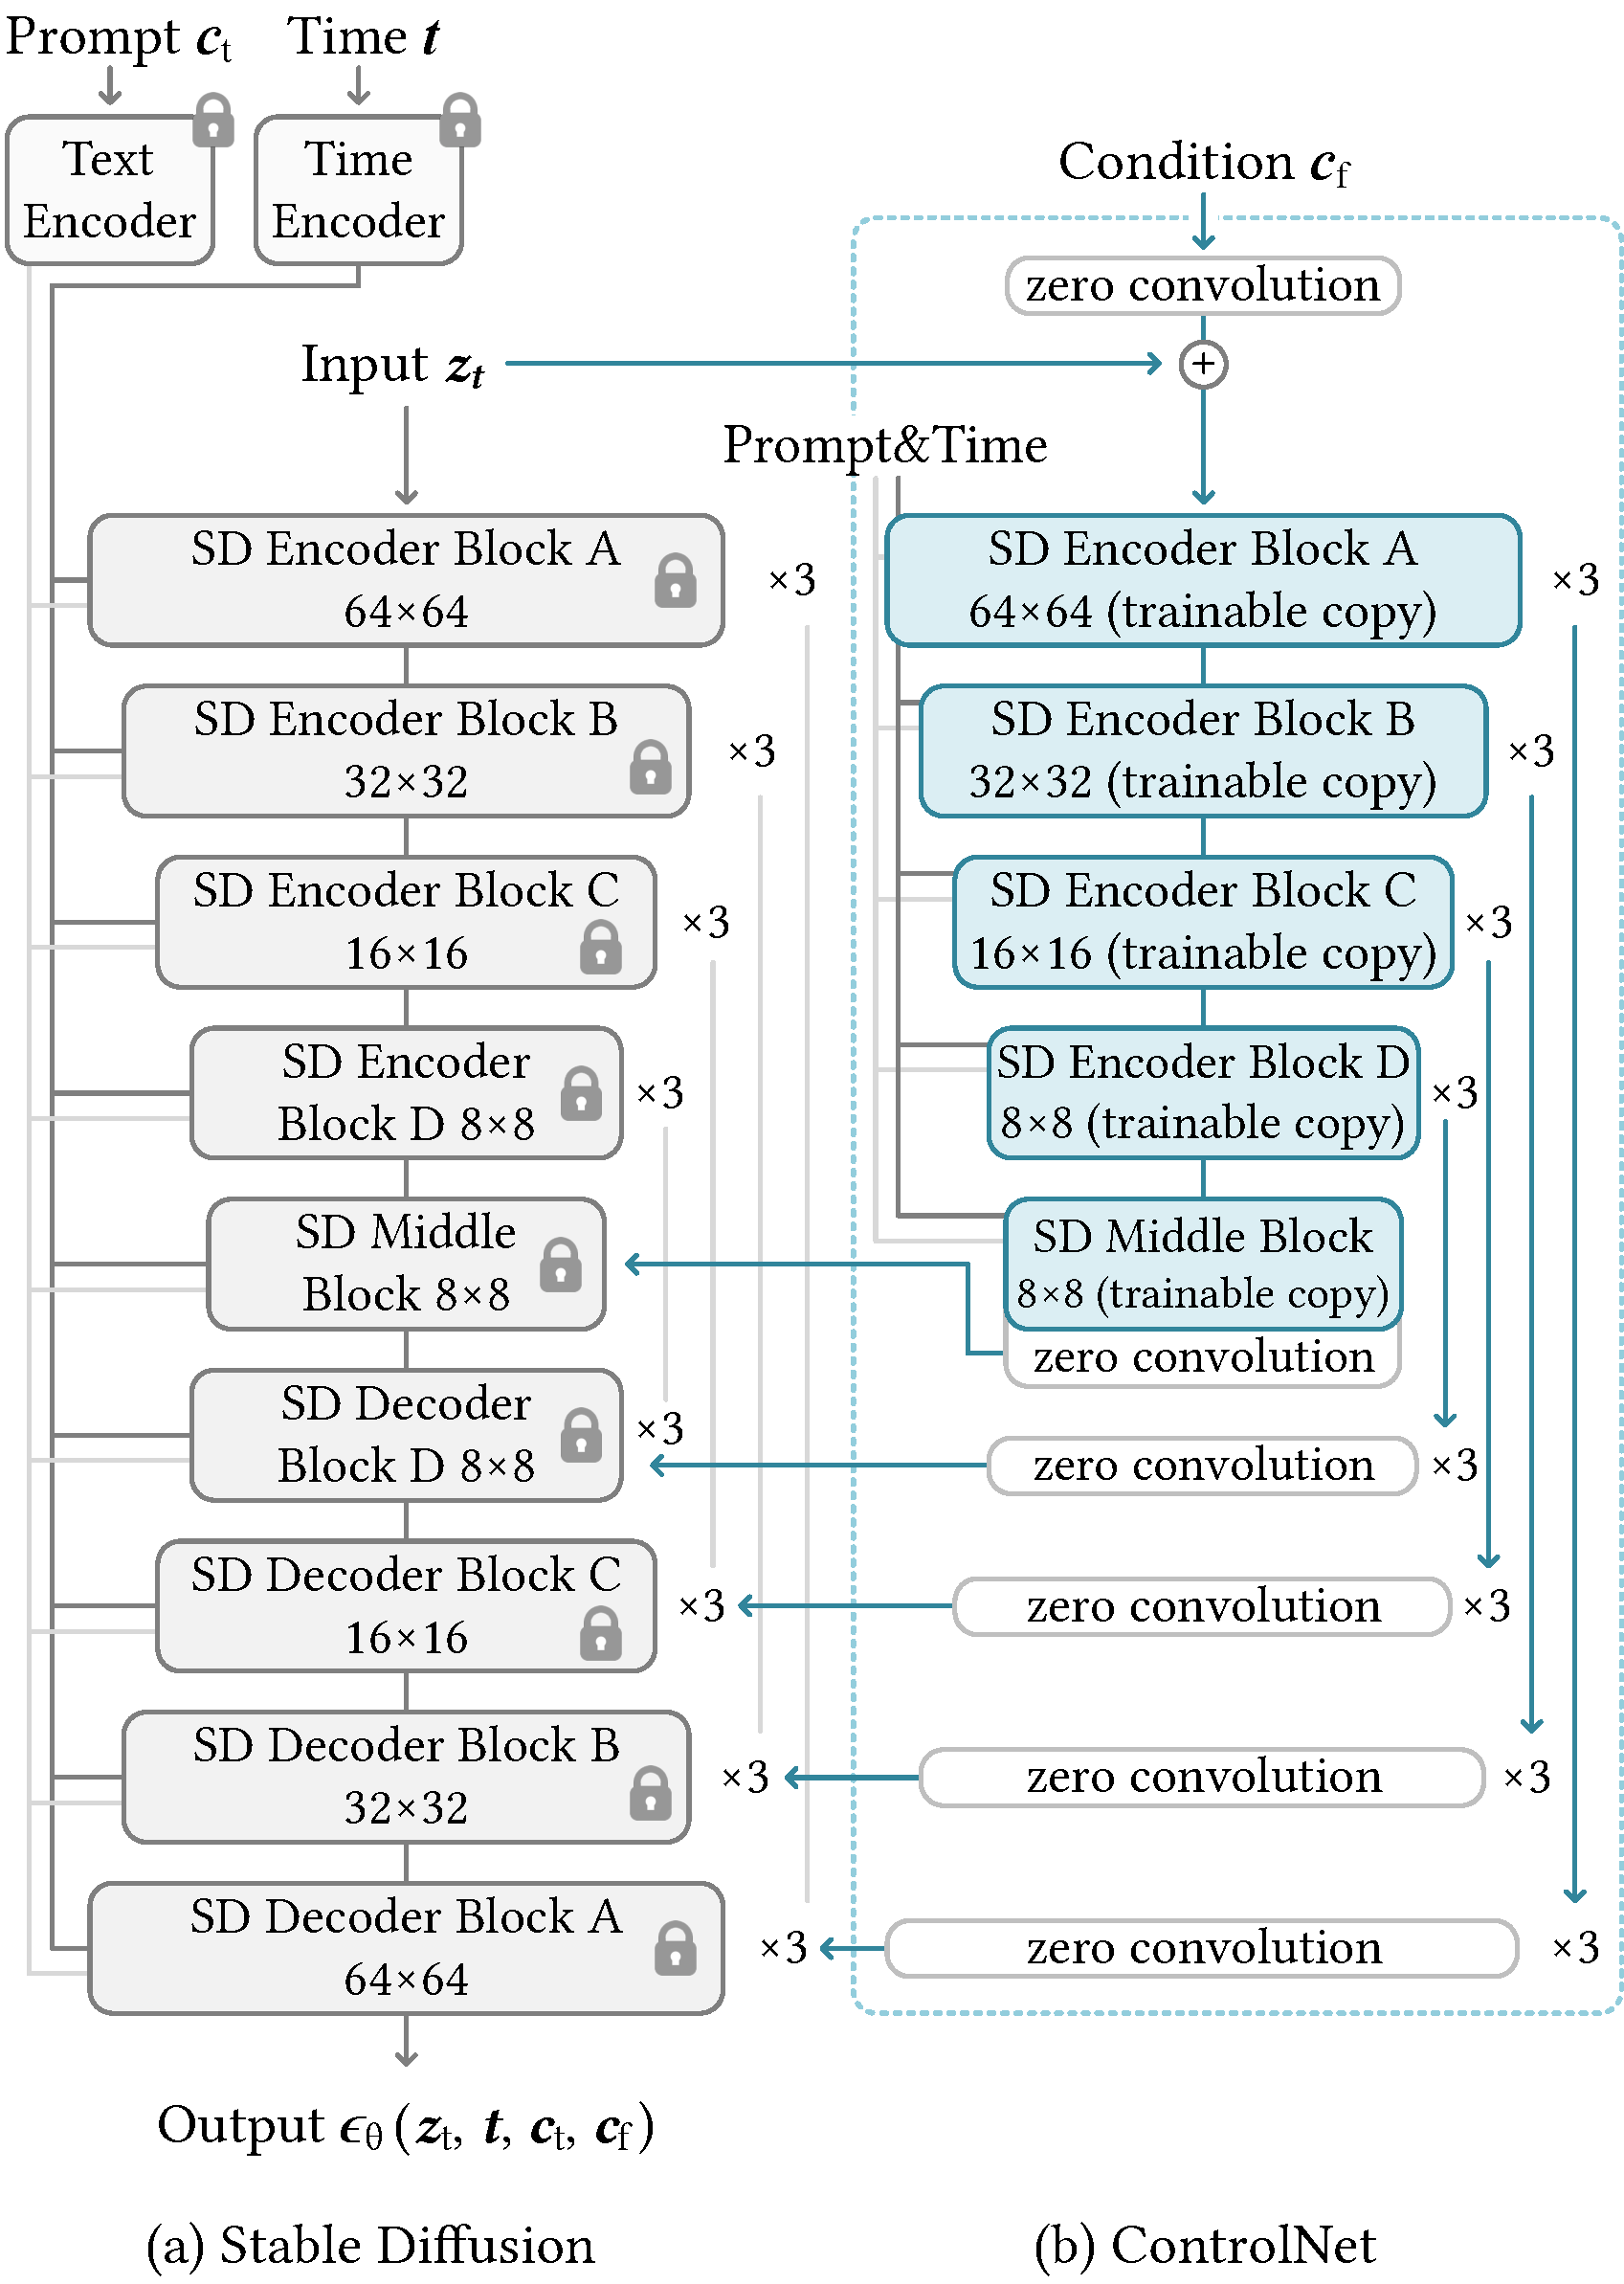
\includegraphics[width=0.5\textwidth]{figures/background/controlnet.pdf}
  \caption{Structure of the ControlNet (right) and the Diffusion Network (left). \cite{zhang2023addingconditionalcontroltexttoimage}}
  \label{fig:controlnet}
  \clearpage
\end{figure}

The outputs from different layers of the ControlNet undergo a zero-convolution layer, a CNN where weights and biases are initialized to zero. However, using Gaussian weights to initialize nodes can degrade the quality. Each output from the ControlNet Encoder Layer is incorporated into the Diffusion Decoder Layers to enhance the diffusion model with additional features. Because the ControlNet maintains a structure similar to its original form, the loss can be computed using the same method for diffusion, leading to efficient training times.

Interestingly, during training, there is a notable fixed point where the diffusion algorithm effectively utilizes the features injected by the ControlNet. This phenomenon is referred to as the \textit{"convergence phenomenon"}.\cite{zhang2023addingconditionalcontroltexttoimage}